\documentclass[convert = false, tikz]{standalone}
\usepackage[utf8]{inputenc}
\usepackage{tikz}
\usetikzlibrary{automata, positioning, arrows}
 
\usepackage{../../../../style_automata}

% arara: pdflatex
% arara: latexmk: { clean: partial }
\begin{document}
    \tikzset{
    node distance=2cm, % specifies the minimum distance between two nodes.
    }
    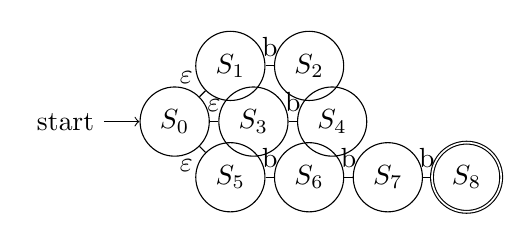
\begin{tikzpicture}
        \node[state, initial] (s0) {$S_0$};
        \node[state, above right of=s0] (s1) {$S_1$};
        \node[state, right of=s1] (s2) {$S_2$};
        \node[state, right of=s0] (s3) {$S_3$};
        \node[state, right of=s3] (s4) {$S_4$};
        \node[state, below right of=s0] (s5) {$S_5$};
        \node[state, right of=s5] (s6) {$S_6$};
        \node[state, right of=s6] (s7) {$S_7$};
        \node[state, accepting, right of=s7] (s8) {$S_8$};
        \draw (s0) edge[above left] node{\(\varepsilon\)} (s1)
        (s1) edge[above] node{b} (s2)
        (s0) edge[above] node{\(\varepsilon\)} (s3)
        (s3) edge[above] node{b} (s4)
        (s0) edge[below left] node{\(\varepsilon\)} (s5)
        (s5) edge[above] node{b} (s6)
        (s6) edge[above] node{b} (s7)
        (s7) edge[above] node{b} (s8);
    \end{tikzpicture}
\end{document}